\chapter{Antecedentes}
\label{chap:stateoftheart}
La individualizaci\'on de filamentos en una imagen es un problema derivado de la obtenci\'on de informaci\'on de filamentos en base a una imagen. Este \'ultimo ha ido variando a medida que la tecnolog\'ia en microscopios ha mejorado, lo que a su vez ha permitido el desarrollo de nuevos m\'etodos. Estos m\'etodos pueden a su vez diferir entre s\'i dependiendo del foco de la informaci\'on que buscan obtener a partir de la imagen, existiendo m\'etodos que se enfocan en reconstruir filamentos discontinuos, a la identificaci\'on de segmentos de filamento para la construcci\'on de las redes que estos conforman, o la individualizaci\'on en s\'i. Independientemente del objetivo de cada m\'etodo, es posible agruparlos en dos categor\'ias: M\'etodos basados en procesamiento de im\'agenes de bajo nivel y m\'etodos basados en optimizaci\'on. Los primeros realizan mayoritariamente operaciones de filtrado sobre la imagen, mientras que los segundos plantean parte de la obtenci\'on de la informaci\'on mediante la resoluci\'on de problemas de asignaci\'on o de minimizaci\'on de funciones.

Entre las herramientas disponibles para los m\'etodos basados en optimizaci\'on, se encuentra la metaheur\'istica {\it Ant Colony Optimization} (ACO), que se basa en el comportamiento de las hormigas al buscar alimento. Esta metaheur\'istica corresponde a la estrategia utilizada en esta investigaci\'on para individualizar filamentos.


\section{M\'etodos basados en procesamiento de im\'agenes de bajo nivel}
\label{sec:NonIndividualizationMethods}

\subsection{SIFNE}
La investigaci\'on de \citet{zhang2017extracting} identifica el problema de discontinuidad de filamentos en una imagen, pudiendo atribuirse esto a factores experimentales como la densidad del componente fluorescente, ruido u otras. En particular, el filamento analizado en esta investigaci\'on corresponde a microt\'ubulos. Para llevar a cabo la reconstrucci\'on de un filamento en base a segmentos, establecen el uso de dos filtros, denominados \textit{Filtro de Transformaci\'on Lineal} (LFT, Linear Filter Transformation) y \textit{Filtro de Transformaci\'on en base a la Orientaci\'on} (OFT, Orientation Filter Transformation). Estos filtros se implementan en un software denominado {\it SIFNE}.
El filtro LFT busca resaltar caracter\'isticas lineales centr\'andose en cada p\'ixel y generando una serie de l\'ineas con radio $r$, buscando la l\'inea que contenga la mayor intensidad, seg\'un se observa en la Figura \ref{fig:MTLFT}. El filtro OFT complementa lo anterior, mediante un criterio de similaridad en la direcci\'on proyectada de los segmentos, un segundo criterio respecto a la distancia entre los extremos finales de cada segmento y un tercer criterio de continuidad, que limita el \'angulo entre el vector proyectado de un extremo y el vector que representa la distancia entre los extremos de cada segmento. Lo anterior se puede observar en la Figura \ref{fig:MTOFT}.

\begin{figure}[h]
        \centering
        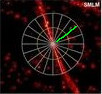
\includegraphics[scale=5]{imagenes/MT-LFT.jpeg}
        \caption[B\'usqueda por l\'ineas con radio $r$ para diferentes \'angulos, según filtro LFT.]{B\'usqueda por l\'ineas con radio $r$ para diferentes \'angulos, según filtro LFT. Fuente: \cite{zhang2017extracting}}.
        \label{fig:MTLFT}
\end{figure}

\begin{figure}[h]
        \centering
        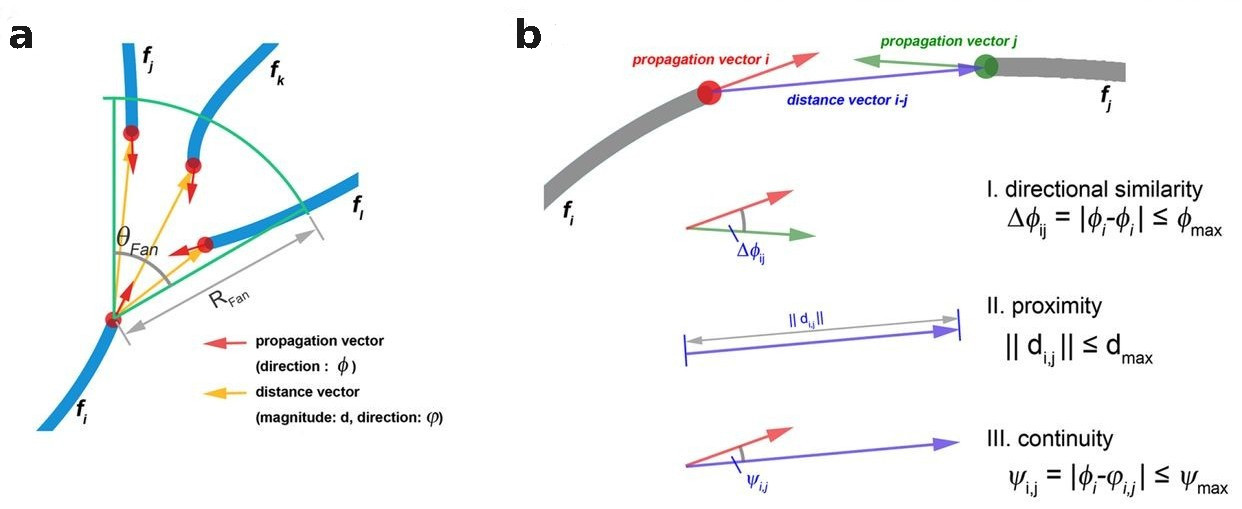
\includegraphics[scale=0.38]{imagenes/MT-OFT.jpeg}
        \caption[Criterios del filtro OFT.]{Criterios del filtro OFT: (a) Vectores de propagaci\'on (rojo) y distancia (amarillo) (b) Ejemplos de criterios de coincidencia de fragmentos de filamento I) Similaridad de direcci\'on, II) Proximidad, III) Continuidad. Fuente: \citet{zhang2017extracting}.}
        \label{fig:MTOFT}
\end{figure}


El fundamento de los criterios de OFT se basa en la asociaci\'on de las caracter\'isticas geom\'etricas como restricciones representativas del comportamiento mec\'anico de los microt\'ubulos. Uno de los objetivos de esta investigaci\'on es permitir el an\'alisis autom\'atico, dada las dificultades que presenta el an\'alisis manual de reconstrucci\'on. % es dificil hacer el analisis de forma manual
%asume non-branching filaments entonces soluciona el caso


% hablar de fibritool, Quantitave IFS y Aliosha
%fibritool
\subsection{FibrilTool}
El trabajo de \citet{boudaoud2014fibriltool} conduce al desarrollo de {\it FibrilTool}, un plugin para el software {\it ImageJ}, utilizado en an\'alisis cient\'ifico de im\'agenes. FibrilTool calcula la orientaci\'on principal y la anisotrop\'ia de estructuras alargadas dentro de una regi\'on de inter\'es seleccionada manualmente. Para esto, utiliza el concepto de tensor nem\'atico, extra\'ido del comportamiento f\'isico de los cristales l\'iquidos. Espec\'ificamente, el tensor nem\'atico es la matriz sim\'etrica $n$ de $2\times2$ construida a partir de un vector unitario $t$, ecuaci\'on \ref{eq:fibritoolTensor}, definido en base a la derivada de primer orden de la intensidad del pixel en $x,y$. %Los componentes de $n$ se pueden observar en la ecuaci\'on \ref{eq:fibritoolComps}.

\begin{equation}
\label{eq:fibritoolTensor}
t = (t_x,t_y) = (
\dfrac{\partial I}{\partial y}, -\frac{\partial I}{\partial x}) / \sqrt{  
(\frac{\partial I}{\partial x})^2 + 
(\frac{\partial I}{\partial y})^2 }
\end{equation}

Luego, a partir de la matriz $n$ (ecuaci\'on \ref{eq:fibritoolComps}) se obtiene su primer vector propio $\Vec{e}_1$ que representa la orientaci\'on principal de los filamentos en el \'area de inter\'es, mientras que la diferencia de los valores propios $\lambda_1$ y $\lambda_2$ ($\lambda_1 > \lambda_2$), denominada $q = \lambda_1 - \lambda_2$, define la anisotrop\'ia.


\begin{equation}
n =
\begin{bmatrix}
(t_x)^2 & t_x \times t_y \\
t_x \times t_y & (t_y)^2 
\end{bmatrix}
\label{eq:fibritoolComps}
\end{equation}

% \begin{subequations}
% Componentes de $n$ para el tensor nem\'atico:
% \begin{align}
%     n_x,x &= (t_x)^2 \\
%     n_y,y &= (t_y)^2 \\
%     n_x,y &= n_y,x = t_x \times t_y
% \end{align}
% \end{subequations}
Los autores de FibrilTool desarrollan este m\'etodo para evitar el uso de derivadas de segundo orden, que presentan sensibilidad al ruido, necesitando de pasos previos en la limpieza de la imagen. Un ejemplo de la ejecuci\'on de FibrilTool sobre una imagen de microt\'ubulos de la planta {\it Arabidopsis Marchantia} se puede observar en  la Figura \ref{fig:FibrilToolexample}.  

\begin{figure}[h!]
        \centering
        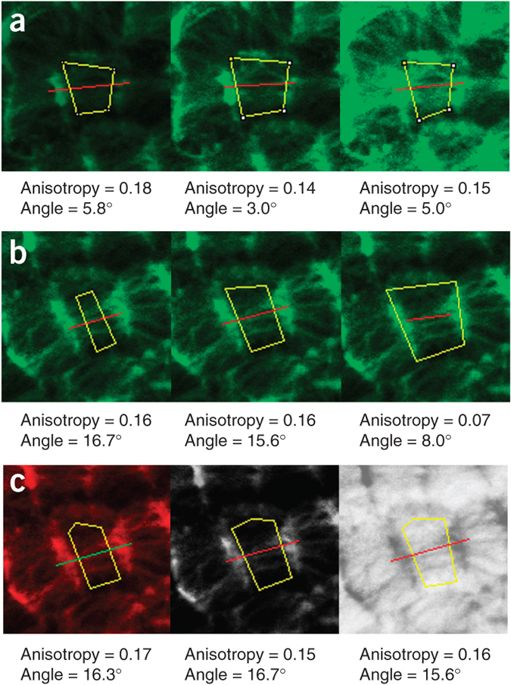
\includegraphics[scale=0.6]{imagenes/fibritool.jpg}
        \caption[\'Area de inter\'es seleccionada manualmente en amarillo, y resultado de FibrilTool en rojo o verde.]{\'Area de inter\'es seleccionada manualmente en amarillo, y resultado de FibrilTool en rojo o verde. Fuente: \citet{boudaoud2014fibriltool}.}
        \label{fig:fibritool}
\end{figure}


%Esta herramienta es el resultado de la investigaci\'on de \citet{boudaoud2014fibriltool}, presentada en la secci\'on \ref{sec:NonIndividualizationMethods}, cuya implementaci\'on consiste en un plugin de facil instalaci\'on para el programa de an\'alisis de im\'agenes ImageJ. FibrilTool permite calcular la anisotrop\'ia de una regi\'on de inter\'es en la que existan filamentos.



A partir del ejemplo, el resultado de FibrilTool se indica mediante una l\'inea de color rojo cuyo \'angulo representa la orientaci\'on promedio de los filamentos en la regi\'on de inter\'es, mientras que el largo es un indicador proporcional a la anistrop\'ia de los filamentos. Adem\'as de la respuesta gr\'afica, FibrilTool genera una salida de datos en formato multi-columna, indicando la orientaci\'on promedio y la anistrop\'ia (definida como $q$) en las columnas 6 y 7 respectivamente. Para el ejemplo, el \'angulo tiene un valor de 52.78\textdegree, con un valor de anistrop\'ia de 0.1493. El \'angulo entregado por la herramienta siempre estar\'a en el rango [90, 90], mientras que la anistrop\'ia puede variar entre 0 y 1, ambos inclusives.

\begin{figure}[h]
    \centering
    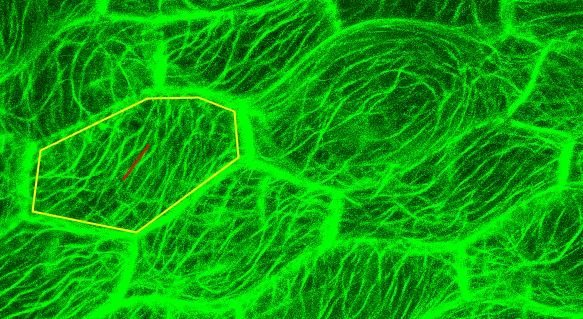
\includegraphics[scale=0.6]{evalImages/fibriltool-c1-mt-GFP-hipocotilo-zoom.png}
    \caption[Ejemplo de FibrilTool en microt\'ubulos]{Uso de FibrilTool en una imagen de microt\'ubulos de la planta {\it Arabidopsis Marchantia}. La secci\'on de inter\'es corresponde al \'area dentro de la regi\'on delimitada en amarillo. La l\'inea roja representa el resultado al ejecutar FibrilTool. El \'angulo de orientaci\'on promedio para este ejemplo es 52.78\textdegree, mientras que la anistrop\'ia reporta un valor de 0.1493. Fuente: Elaboraci\'on Propia.}
    \label{fig:FibrilToolexample}
\end{figure}

% Fibriltool batch mention
Debido a que el proceso para obtener un resultado a partir de FibrilTool considera una sola \'area de inter\'es, los autores desarrollaron una versi\'on denominada {\it FibrilTool Batch} \citepxl{marion_louveaux_2018_2528872}, la que permite la creaci\'on de m\'ultiples regiones de inter\'es para ser calculadas.
% Image filename
%N° de ROI
% coord x,y of the ROI center
% area
% average fibril orientation [-90,90]°
% anisotropy [0,1]

\subsection{IFS}
% Quantitative IFS
Una investigaci\'on que propone la individualizaci\'on de segmentos de filamentos es \citet{qiu2014quantitative}, la que plantea un filtro de detecci\'on de caracter\'isticas de 6 pasos m\'as un algoritmo llamado \textit{SBDA} que busca eliminar segmentos de filamentos menores a 2 p\'ixeles (Figura \ref{fig:IFS}), cuya implementaci\'on de denomina {\it IFS}. La individualizaci\'on de segmentos de filamentos entrega informaci\'on morfol\'ogica de un segmento con respecto a su entorno, se\~nalando si se encuentra en estado de aislaci\'on, intersectado, bifurcado o en superposici\'on con otro segmento de filamento.

%describir filtros, intensidad es con fibre coefficient
Las 6 etapas del filtro consideradas en este m\'etodo consisten en 4 etapas de an\'alisis de la imagen y 2 de an\'alisis topol\'ogico que se resumen en lo siguiente:

\begin{enumerate}
    \item Depuraci\'on de la imagen: El primer filtro comienza por reducir el ruido y realzar el contraste de la imagen, aumentando la intensidad de los p\'ixeles que est\'en sobre un umbral, al mismo tiempo que se descartan los p\'ixeles que se encuentren debajo del mismo umbral.
    \item Filtro de informaci\'on estructural: El segundo paso consiste en filtrar informaci\'on estructural, que se basa en los valores propios de la matriz Hessiana, buscando descartar objetos en la imagen que no correspondan a una figura tubular.
    \item Eliminaci\'on de se\~nales d\'ebiles: El tercer filtro ejecuta una limpieza de estructuras con una intensidad baja y/o aisladas, de las que puede concluirse que no corresponden a elementos en el plano focal de inter\'es.
    \item Generaci\'on de esqueleto: Finalmente dentro del an\'alisis sobre la imagen, el filtro de esqueletonizaci\'on realiza un adelgazamiento de la imagen, en el que cada estructura pasa a tener 1 p\'ixel de ancho, facilitando el an\'alisis topol\'ogico posterior.
    \item Clasificaci\'on topol\'ogica y algoritmo SBDA: Consiste en el an\'alisis a nivel de p\'ixel y su vecindario de 8 p\'ixeles alrededor para determinar si este corresponde a un punto aislado, al final de un fragmento de filamento, a un punto interior de un filamento, o a una junci\'on de filamentos. Seguido de aquello, el algoritmo SBDA realiza otro an\'alisis topol\'ogico a nivel de p\'ixel que borra los segmentos menores a 3 p\'ixeles, adem\'as de realizar los calculos de distancia de cada segmento/fragmento.
    \item Reconstrucci\'on: Para finalizar el an\'alisis topol\'ogico y el proceso de filtrado, se lleva a cabo una combinaci\'on de segmentos para construir los filamentos bas\'andose en el par\'ametro $W$, llamado \textit{ancho efectivo}, cuyo valor define si la uni\'on de 2 o m\'as segmentos se trata de una bifurcaci\'on, una intersecci\'on o un solapamiento. 
\end{enumerate}

\begin{figure}[h!]
        %\centering
        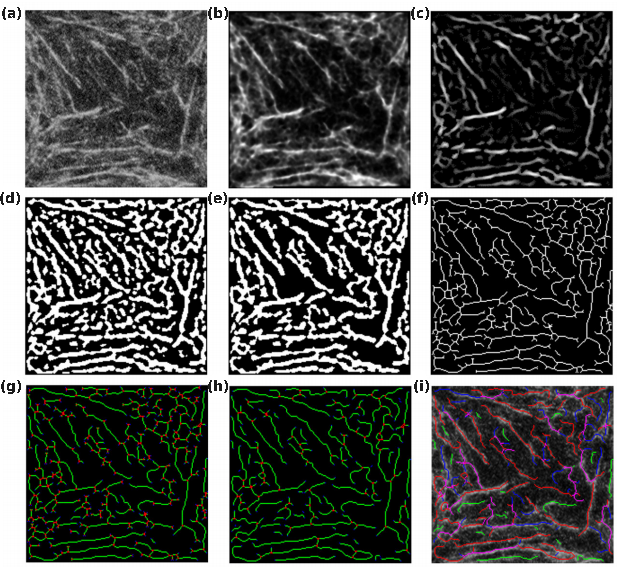
\includegraphics[scale=0.75]{imagenes/QuantitativeIFS.png}
        \caption[Etapas de individualizaci\'on de filamentos de \cite{qiu2014quantitative}.]{Etapas de individualizaci\'on de filamentos de \cite{qiu2014quantitative}. (a): Imagen de red de fibras de un osteoblasto. (b, c, d, e, f): Filtros de limpieza, tubularidad, segmentaci\'on, conectividad y esqueletonizaci\'on. (g): Clasificaci\'on topol\'ogica de intersecciones a nivel de p\'ixel. (h): Resultado de algoritmo SBDA. (i): Individualizaci\'on de segmentos de filamentos seg\'un forma estructural: aislado (verde), solapado (morado) u otro (azul). Fuente: \cite{qiu2014quantitative}.}
        \label{fig:IFS}
\end{figure}
%describir SBDA, el analisis es a nivel de pixel

% se mide caracteristicas geometricas, como largo, distribucu\'on de la orientaci\'on, y como los resultados son afectados por el ruido.
Como resultados de \cite{qiu2014quantitative}, adem\'as de la informaci\'on morfol\'ogica, se obtienen caracter\'isticas geom\'etricas como el largo de los segmentos de  filamentos y la distribuci\'on de la orientaci\'on de los segmentos, as\'i como el cambio de estos valores para variaciones en la relaci\'on entre la se\~nal y el ruido de la imagen.

\subsection{Marco de An\'alisis de Im\'agenes de Filamentos de Actina}
%\smallskip
La investigaci\'on de \citet{alioscha2016robust} presenta un marco para el an\'alisis de im\'agenes con la finalidad de identificar filamentos de actina, mediante una combinaci\'on de filtros con un algoritmo de uni\'on de segmentos. La propuesta inicial se basa en que una imagen puede ser separada en 3 componentes: el fondo o {\it background} de la imagen, los filamentos y el ruido. Para obtener la imagen que contiene los filamentos y descartar en mayor medida el ruido, los autores utilizan la libreria MCALab en MATLAB. Luego, buscan intensificar los p\'ixeles que corresponden a los filamentos, para lo cual aplican 3 filtros: un filtro Gaussiano, un filtro Laplaciano y un filtro Gaussiano direccional, obteniendo como resultado lo que se muestra en la Figura \ref{fig:AlioshaRobust}.

\begin{figure}[h]
    \centering
    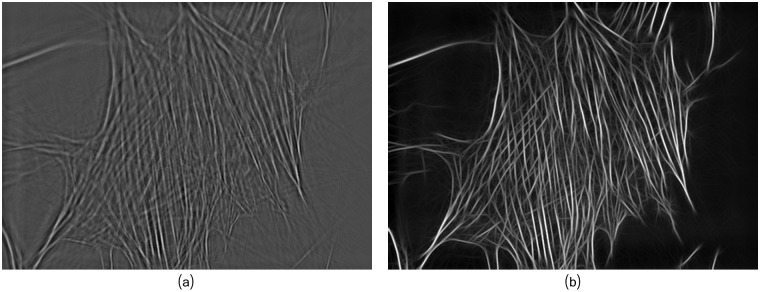
\includegraphics[scale=2]{imagenes/Aliosha2016-GaussLaplFilters.jpg}
    \caption[Aplicaci\'on de filtros posterior a la segmentaci\'on.]{A partir de la segmentaci\'on obtenida con la libreria MCALab (a), se aplican los filtros Gaussiano, Laplaciano y Gaussiano direccional para obtener una intensificaci\'on de los filamentos (b). Fuente: \citet{alioscha2016robust}.}
    \label{fig:AlioshaRobust}
\end{figure}

%\vspace{-1cm}

El paso siguiente es la aplicaci\'on de un detector de l\'ineas multi-escala, que busca determinar la pertenencia de un p\'ixel a una l\'inea, que varia su grosor y \'angulo dependiendo del tama\~no/escala del vecindario elegido. Las l\'ineas var\'ian en su grosor $s \in [1,W]$, con $W$ el grosor esperado de una fibra de actina, as\'i como en su \'angulo, que varia de forma discreta entre 0 y 180\textdegree. El detector de l\'ineas asigna una puntuaci\'on que determina la probabilidad del p\'ixel a pertenecer a una de las l\'ineas. Lo anterior entrega como resultado candidatos de segmentos de l\'ineas. Para elegir a un candidato como segmento de l\'inea definitivo, la idea principal es recorrer los p\'ixeles en secuencia y ajustar las l\'ineas candidatas usando el m\'etodo de m\'inimos cuadrados hasta que un umbral de error es sobrepasado. Por cada vez que se sobrepasa el umbral de error, se comienza la elecci\'on de un nuevo segmento de l\'inea para los p\'ixeles que siguen. Si el candidato de segmento de l\'inea tiene un largo $l < L$, se descarta. $L$ es un par\'ametro definido emp\'iricamente.
% esto arroja candidatos de segmentos de l\'ineas -> elegir segmentos de l\'ineas
% despues hay merge de segmentos l\'ineas -> segmentos de filamentos, fibras en este caso

Finalmente, para construir las fibras de actina, los segmentos de l\'inea elegidos en el paso anterior son unidos entre s\'i mediante una ventana de largo $L$, en la que dos segmentos de l\'inea se superpongan y no tengan una diferencia entre sus \'angulos mayor al umbral $T_{\theta}$. 
%\cite{asgharzadeh2018computational}

Otras investigaciones similares que siguen un enfoque basado principalmente en procesamiento de im\'agenes de bajo nivel son \citet{doi:10.1021/ma502264c},\citet{lichtenstein2003quantitative} y \citet{asgharzadeh2018computational}. En general, los trabajos desarrollados bajo este enfoque requieren del uso o sintonizaci\'on de m\'ultiples par\'ametros.


%la dificultad para identificar correctamente un filamento de otro, en los casos de  superposici\'on, fragmentaci\'on, o variaciones de intensidad en la imagen...


\section{M\'etodos basados en optimizaci\'on}
\label{sec:OptiMethods}

\subsection{Restricciones Geometricas para Segmentar Estructuras Alargadas}
En la segunda categor\'ia, \citet{cerda2014geometrical} plantea la identificaci\'on de segmentos de filamentos como un problema de asignaci\'on, utilizando las medidas de distancia Euclidiana y angular como restricciones, y el algoritmo h\'ungaro para su resoluci\'on.

\subsection{SOAX}
%SOAX, extraccion y cuantifiacion de la red
Por su parte, la investigaci\'on de \citet{xu2015soax} llamada SOAX, emplea curvas param\'etricas de contorno abierto (SOAC, {\it Stretching Open Active Contour}) en conjunto con una funci\'on de minimizaci\'on para obtener un grupo acotado de redes de filamentos, entre las que el usuario puede elegir una, con la finalidad de realizar un an\'alisis posterior. Las curvas param\'etricas de contorno abierto son reguladas por los par\'ametros $\tau$ y $K_{str}$. El par\'ametro $\tau$ fija el umbral de intensidad que permite discriminar los puntos en la imagen donde existen m\'aximos locales, a partir de los cuales puede comenzar el recorrido de una curva SOAC.
%desde el que se inicializa una SOAC, lo que entrega los puntos de intensidad m\'aximos locales de la imagen para la inicializaci\'on. 
Por su parte, el par\'ametro, $K_{str}$ es el factor que regula la elongaci\'on/evoluci\'on de cada curva param\'etrica de contorno abierto (SOAC). Una vez concluida la inicializaci\'on y evoluci\'on de curvas SOAC, se identifican las junciones/intersecciones generadas entre diversas curvas SOAC, agrup\'andose seg\'un su cercan\'ia. Lo anterior se puede observar en la Figura \ref{fig:SOAX}.

\begin{figure}[h]
        %\centering
        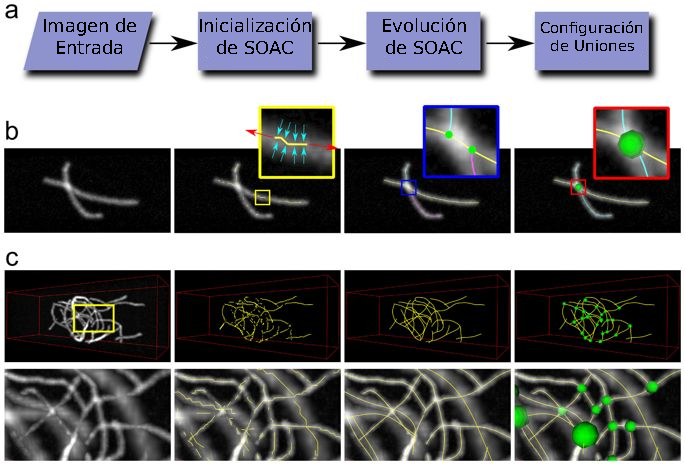
\includegraphics[scale=0.7]{imagenes/SOAX_translated.png}
        \caption[Etapas de SOAX.]{Etapas de SOAX: A partir de los puntos de alta intensidad se inicializan curvas param\'etricas de contorno abierto (SOAC), las que crecen, generando intersecciones entre ellas. Finalmente, se agrupan las intersecciones más cercanas. Fuente: \citet{xu2015soax}.}
        \label{fig:SOAX}
\end{figure}

La funci\'on de minimizaci\'on que los autores denominan como  \textit{F-Function}, $F = -L_{total} + {c}\cdot L_{<t}$, se encuentra definida por otros 2 par\'ametros: el factor $c$ ($c > 1$) que regula la penalizaci\'on de las SOACs con bajo \textit{Signal to Noise Ratio (SNR)}, y el umbral $t$, que define el valor mínimo de SNR necesario para no descartar una SOAC. El umbral $t$ se ve reflejado en $L_{<t}$ dentro de la \textit{F-Function}, como el largo de SOACs en una regi\'on de la imagen con SNR por debajo de $t$, y que ser\'an penalizados dado que son calificados como de baja certeza. $L_{total}$ representa el largo total de las SOACs en el resultado final.

% \begin{equation}
%   \label{eq:FFunction}
%     F = -L_{total} + {c}\cdot L_{<t} 
% \end{equation}


%La herramienta descrita en la investigaci\'on denominada SOAX \citepxl[]{xu2015soax}, presentado en la secci\'on \ref{sec:OptiMethods}, pudo ser construida para realizar una evaluaci\'on, utilizando la imagen de ejemplo provista por los autores. Esta imagen se puede observar en la Figura \ref{fig:SOAXexample}.

%Para la construcci\'on de SOAX es necesario compilar las herramientas ITK y VTK, las que cuentan con m\'ultiples versiones, no existiendo claridad de cual es el rango de versiones para las que es posible construir SOAX y as\'i obtener la herramienta con todas las funcionalidades descritas por los autores. Lo anterior se menciona debido a que intentos posteriores de evaluaci\'on con im\'agenes distintas a la del ejemplo no fueron reconocidas por el programa.

La ejecuci\'on de SOAX utilizando una imagen de microt\'ubulos en la planta {\it Arabidopsis Marchantia}

\begin{figure}[h]
    \centering
    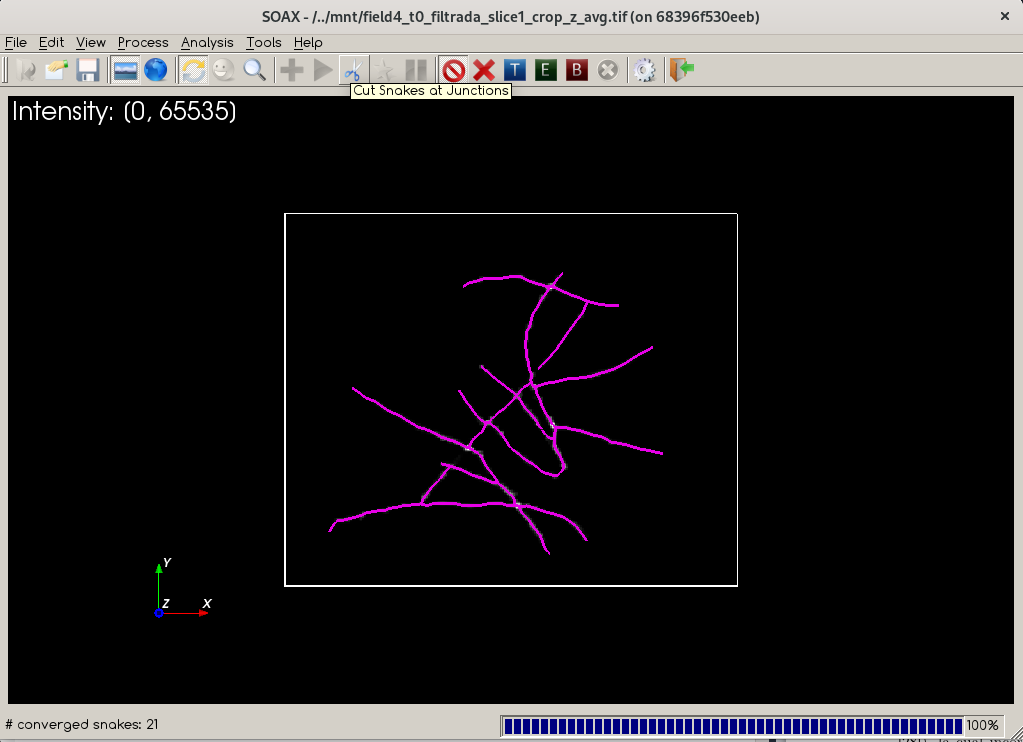
\includegraphics[scale=1]{evalImages/field4-soax.png}
    \caption[Imagen de ejemplo de SOAX]{Imagen recortada con microt\'ubulos de {\it Arabidopsis Marchantia} para el ejemplo de SOAX. Fuente: Paula Llanos, PhD.}
    \label{fig:SOAXexample}
\end{figure}

 


En base a la imagen de ejemplo se pueden obtener m\'ultiples caracter\'isticas de la red de filamentos, a partir de las curvas param\'etricas SOAC identificadas. Estas caracter\'isticas son la rotaci\'on esf\'erica, la orientaci\'on, la densidad de puntos, curvatura y largo de estas. A su vez, SOAX tambi\'en identifica las intersecciones de las curvas SOAC, lo que se indica en la Figura \ref{fig:SOAXexampleComputed}, como los puntos verdes.


Dado que el enfoque de la investigaci\'on de SOAX se encuentra en obtener un an\'alisis cuantitativo de la red de filamentos, las curvas SOAC pueden coincidir con un filamento o simplemente corresponder a un segmento de filamento, sin existir una diferencia entre ambas. En cuanto a los par\'ametros, SOAX presenta 26 campos para poder modificar valores, con 2 opciones adicionales del tipo booleana.

\begin{figure}[h]
    \centering
    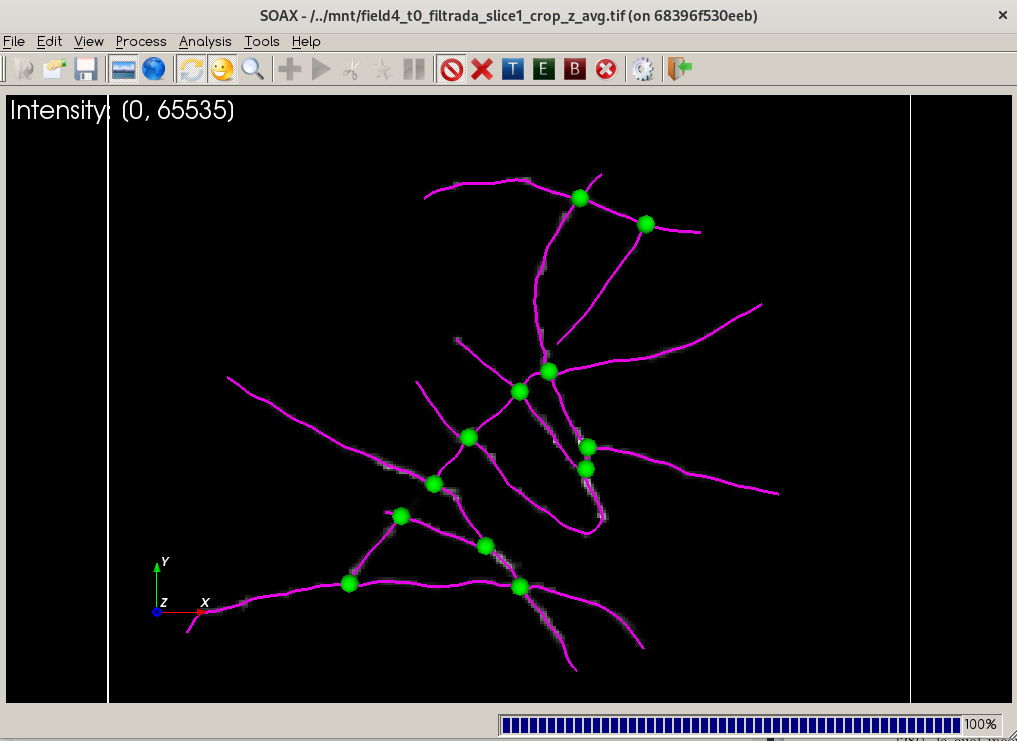
\includegraphics[scale=0.4]{evalImages/field4-nodes-soax.png}
    \caption[Imagen de ejemplo procesada con SOAX]{Resultado de SOAX al procesar la imagen recortada con microt\'ubulos de {\it Arabidopsis Marchantia}. Tras aplicar la opci\'on de corte de curvas param\'etricas, y la posterior selecci\'on de la opci\'on de agrupar curvas param\'etricas, es posible observar las intersecciones en color verde. Fuente: Elaboraci\'on Propia.}
    \label{fig:SOAXexampleComputed}
\end{figure}


Los mismos autores de SOAX crearon una extensi\'on, denominada TSOAX \citepxl{xu2018automated}, la cual incorpora la posibilidad de analizar y extraer redes de filamentos a partir de un conjunto de im\'agenes que reflejen la evoluci\'on de los filamentos en el tiempo. Los pasos utilizados para la construcci\'on de SOAX y TSOAX  pueden encontrarse en los archivos del tipo {\it Dockerfile} disponibles en el repositorio de esta tesis para su reproducci\'on.
%, siendo la mayor diferencia la existencia de un nuevo par de par\'ametros, los que se deshabilitan para realizar una evaluaci\'on que sea m\'as similar al comportamiento esperado de SOAX.

%La similaridad entre SOAX y TSOAX permite a los autores indicar que el mismo manual de usuario es aplicable a ambas herramientas.
%que permiten seguir filamentos en distintos tiempos, as\'i como llevar a cabo la agrupaci\'on de curvas param\'etricas 


\subsection{DeFiNe}
En esta categor\'ia tambi\'en se incluye \citet{breuer2015define}, que en base a un grafo no dirigido con pesos que representa la red de filamentos, realiza la individualizaci\'on de estos. El uso de un grafo como dato de entrada permite representar a cada filamento mediante un conjunto de aristas adyacentes en el grafo. Esto permite que la b\'usqueda e individualizaci\'on de filamentos, con un segmento de filamento representado por una o m\'as aristas del grafo, sumado a las restricciones que plantea el autor, sea tratado como un problema de {\it Set Cover} \citepxl{caprara2000algorithms}. La definici\'on de {\it Set Cover} es:

\begin{quote}
Dado un conjunto de elementos, denominado universo, y $n$ conjuntos cuya unión comprende el universo, el {\it Set Cover Problem} consiste en identificar el menor n\'umero de conjuntos cuya unión a\'un contiene todos los elementos del universo.
\end{quote}

%En particular, el m\'etodo {\it FCP} presentado en la secci\'on \ref{Antecedentes}, utiliza s\'olo el grosor como caracter\'istica en la etapa de asignaci\'on de pesos a las aristas del grafo, lo que es usado en la funci\'on de minimizaci\'on del problema de optimizaci\'on planteado por ellos. En la etapa de selecci\'on del subconjunto de caminos, el mismo m\'etodo desarrolla una heur\'istica que utiliza {\it BFS} en conjunto con el \'angulo de deflexi\'on entre aristas. El mismo m\'etodo evita realizar un recorrido de grafos, al buscar las combinaciones de caminos del subconjunto P' que dan lugar a uno o m\'as filamentos mediante la minimizaci\'on de un {\it Set Cover}. 

%representa un camino en este grafo, y los conjuntos de caminos 
\medskip
%Todos estos enfoques, cuya entrada principal de datos son las im\'agenes etiquetadas a trav\'es de marcadores fluorescentes, 
% basados en grafos

El programa \texttt{DeFine} desarrollado en \citet{breuer2015define} describe el problema de individualizaci\'on de filamentos como un problema de b\'usqueda de conjuntos de aristas en un grafo. En esta investigaci\'on, un filamento es representado por un conjunto de aristas, denominado como un camino. Los autores de esta investigaci\'on se basan inicialmente en un problema del tipo {\it Path Cover} \citepxl{ntafos1979path}, extendiendo la definici\'on de {\it Path Cover} mediante la asignaci\'on de un peso a cada segmento/arista del grafo, para calcular la {\it aspereza} o diferencia de homogeneidad en un camino. El c\'alculo del peso a lo largo de un camino es lo que permite individualizar filamentos, siendo el peso un reflejo del grosor o intensidad de una arista.
%, o tambi\'en puede ser calculado respecto al \'angulo entre aristas.
Este problema particular es llamado {\it Filament Covering Problem} (FCP) y los autores demuestran que es NP-Hard, por lo que proponen un algoritmo de aproximaci\'on mediante {\it Set Cover}, cuyo objetivo es que cada arista pertenezca al menos a un camino (conjunto de aristas).

La adaptaci\'on a lo definido por {\it FCP} es: 
\begin{quote}
Sea el universo $U$ conformado por las aristas del grafo, y un conjunto $S$, conformado por conjuntos de aristas, cada uno con costo $c_s$, $s \in S$:

Encontrar un subconjunto $S_{set} \subseteq S$ con costo m\'inimo (o promedio, dependiendo de la forma en que se calcula la aspereza) tal que cada elemento en $U$ este cubierto al menos una vez.
\end{quote}

Los autores de DeFiNe demuestran que el FCP es NP-Hard en grafos, debido a la relaci\'on entre el n\'umero de nodos y el conjunto total de caminos posibles. Esta relaci\'on implica que al aumentar el n\'umero de nodos, el conjunto total de caminos en un grafo, definido como $P$, crece de forma exponencial. Para esta situaci\'on, los autores de DeFiNe prueban que el FCP en \'arboles es soluble en tiempo polinomial, bas\'andose en \citet{lin2006vertex}. La complejidad computacional para resolver el FCP en \'arboles es de $\mathcal{O}(n^{4})$ para caminos que no comparten nodos o aristas, es decir, no se superponen. Para permitir caminos que se superponen se agrega el par\'ametro $k$ que define el n\'umero m\'aximo de superposiciones de caminos en una arista, quedando la complejidad computacional igual a $\mathcal{O}(n^{2k+2})$.


%aca entran las formas de obtener esos arboles simples y bosques, con las heuristicas de define
DeFine propone 2 heur\'isticas para construir \'arboles de los cuales se puedan extraer un subconjunto $P' \in P$ representativo de caminos simples: recorrer el grafo por su anchura ({\it Breadth-First Search}), deteni\'endose al momento en que el \'angulo de deflexi\'on entre aristas adyacentes supere los 60\degree, o generar caminos a partir de 100 \'arboles de expansi\'on m\'inima aleatoria ({\it RMST}), aportando cada uno con $N(N-1)/2$ caminos no triviales y sin direcci\'on. 


El subconjunto $P'$ constituye los datos de entrada del problema de {\it Set Cover}, el que se resuelve a trav\'es de un algoritmo de aproximaci\'on lineal fraccional binario \citepxl{breuer2015define}, en el que al subconjunto $P'$ se le aplica la funci\'on objetivo, para encontrar los miembros de $p \in P'$ que mejor minimicen la diferencia de homogeneidad en sus caminos. La restricci\'on de lo anterior es que cada arista del grafo pertenezca a lo menos a un camino. El flujo de decisiones para generar el subconjunto de caminos puede observarse en la Figura \ref{fig:define-set-cover}.

\begin{figure*}[h]
    \centering
    \label{fig:flujo-expected-define}
    \begin{subfigure}[t]{\textwidth}
        \centering
        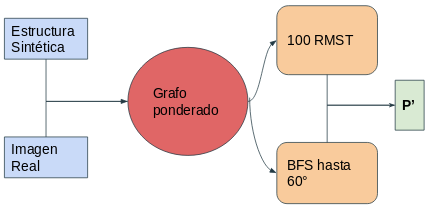
\includegraphics[scale=0.5]{imagenes/flujoDefine.png}
        \caption{Entrada de datos y elecci\'on de subconjunto de caminos {\bf P'} en DeFine.}
        \label{fig:define-set-cover}
    \end{subfigure}%
    \vskip\baselineskip
    \begin{subfigure}[t]{\textwidth}
        \centering
        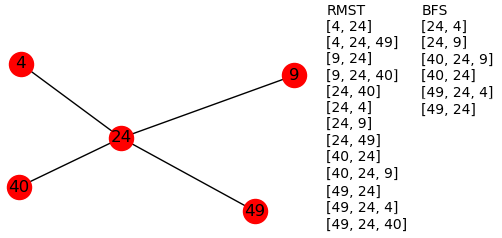
\includegraphics[scale=0.8]{imagenes/BFSvsRMSTpaths.png}
        \caption{Subconjunto {\bf P'} para el grafo de 5 nodos a la izquierda, utilizando la opci\'on de 100 {\it RMST} o heur\'istica de {\it BFS} que corta el camino al encontrar un \'angulo de deflexi\'on mayor a 60\degree entre aristas adyacentes.  }
        \label{fig:subconjunto-p-prima-caminos-posibles}
    \end{subfigure}
    \caption[Extracci\'on de caminos para formar P' en DeFiNe.]{(a) A partir de un grafo ponderado proveniente de una estructura sint\'etica o de una imagen real, se elige {\bf P'} entre los $N(N-1)/2$ caminos no triviales y sin direcci\'on que aporta cada uno de los 100 \'arboles de expansi\'on m\'inima aleatoria ({\it RMST}), o los caminos resultantes de la heur\'istica de b\'usqueda por anchura ({\it BFS}) con interrupci\'on al dar con una arista que tenga un \'angulo superior a 60\degree. (b) Subconjunto {\bf P'} de P, para el grafo de 5 nodos de ejemplo a la izquierda. Fuente: \citet{breuer2015define}.}
    \end{figure*}
    
    
%Este enfoque faculta que al tener un grafo que representa la red de filamentos, como en la figura \ref{Fig1d}, sea posible llegar a resultados como los que aparecen en las figuras \ref{Fig2a} o \ref{Fig2b} a trav\'es de la minimizaci\'on de la diferencia de homogeneidad del peso de las aristas en un camino, y de restricciones a las uniones entre las mismas. 

Cabe destacar que el {\it FCP} s\'olo utiliza 2 caracter\'isticas independientes para describir los segmentos de los filamentos, siendo el \'angulo de deflexi\'on entre aristas usado en la etapa de selecci\'on de subconjuntos de caminos s\'olo si es seleccionada la heur\'istica {\it BFS}, y el grosor o intensidad, empleado para describir el peso de las aristas. En el caso de la heur\'istica de {\it RMST}, se asignan pesos aleatorios uniformemente distribuidos a las aristas, por lo que no hay uso de caracter\'isticas asociadas a los filamentos.

\vspace{1cm}

En el caso de los m\'etodos basados en optimizaci\'on, la mayor cr\'itica es su costo computacional, el que aumenta a medida que se complejiza, limitando en parte aquel enfoque. Se debe agregar que los par\'ametros utilizados por estas t\'ecnicas (\'angulos o  distancias m\'aximas entre filamentos) son complejas de obtener de los expertos directamente. Sin embargo, una de sus ventajas es que automatizan la recuperaci\'on de informaci\'on incluyendo una mayor cantidad de propiedades a cada arista. 


%resolucion, cantidad parametros, descriptores, costo computacional
En resumen, el problema de identificar filamentos en im\'agenes de microscop\'ia esta limitado por la resoluci\'on, y los problemas de m\'ultiples par\'ametros a ajustar, para los m\'etodos basados en procesamiento de im\'agenes de bajo nivel, el costo computacional en los m\'etodos basados en optimizaci\'on, y falta de descriptores cuantitativos en ambas. La revisi\'on bibliogr\'afica da cuenta tambi\'en de pocas herramientas disponibles. Todo lo anterior implica que parte del an\'alisis deba ser manual, lo que para grandes cantidades de datos, hace los estudios m\'as propensos a errores. 


\section{Generaci\'on de un grafo desde una imagen}
\label{sec:genGrafFromImage}
%La falta de herramientas analíticas para cuantificar las estructuras sigue siendo un cuello de botella, ya que el análisis manual de grandes conjuntos de datos requiere una gran cantidad de tiempo y son propensos a sesgos y errores.
%Por otra parte, la soluci\'on a problemas de superposici\'on se soluciona mediante la sintonizaci\'on de par\'ametros, los que var\'ian dependiendo de la c\'elula observada. En el caso del uso de \textit{thinning} en una imagen, la informaci\'on respecto al grosor de la estructura se pierde.
El uso de grafos para la individualizaci\'on de filamentos implica la necesidad de obtener el grafo a partir de una imagen para luego realizar su an\'alisis. Algunas de las dificultades involucradas en la obtenci\'on de un grafo se relacionan al ruido y la resoluci\'on de la imagen. Un ejemplo de aquello se observa en la Figura \ref{fig:NoConsensoGeneral}.

\begin{figure*}[h]
    %\centering
    \begin{subfigure}[h]{\textwidth}
        \centering
        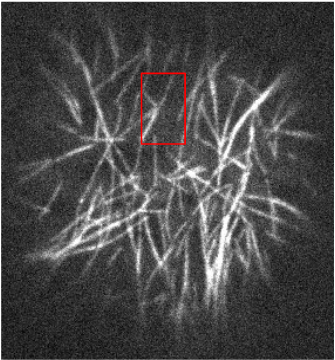
\includegraphics[scale=0.5]{imagenes/NoConsenso.png}
        \caption{Microt\'ubulos en planta {\it Marchantia}.\\Fuente: Paula Llanos}
        \label{fig:NoConsensoGeneral}
    \end{subfigure}
    \vskip\baselineskip
    \begin{tabular}{c c c}
    
        \begin{subfigure}[t]{0.3\textwidth}
            \centering
            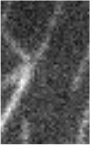
\includegraphics[height=1.6in]{imagenes/NoConsenso2.png}
            \caption{Secci\'on resaltada en rojo de (a)} %\ref{fig:NoConsensoGeneral}
            \label{fig:NoConsensoRect}
        \end{subfigure}
        &
    
        \begin{subfigure}[t]{0.3\textwidth}
            \centering
            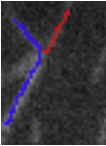
\includegraphics[height=1.6in]{imagenes/NoConsenso3.png}
            \caption{Opci\'on 1 de microt\'ubulos en (b)} %\ref{fig:NoConsensoRect}
            \label{fig:NoConsensoOpcion1}
        \end{subfigure}
        &
    
        \begin{subfigure}[t]{0.3\textwidth}
            \centering
            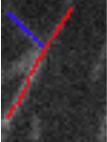
\includegraphics[height=1.6in]{imagenes/NoConsenso4.png}
            \caption{Opci\'on 2 de microt\'ubulos en (b)}
            \label{fig:NoConsensoOpcion2}
        \end{subfigure}
    \end{tabular}
    
    \caption[Dificultad de individualizaci\'on que enfretan los expertos al analizar manualmente una imagen de filamentos.]{Dificultad de individualizaci\'on que enfretan los expertos al analizar manualmente una imagen de filamentos, en particular, microt\'ubulos. Fuente: Elaboraci\'on Propia.}
    \label{fig:NoConsenso}
\end{figure*}

%El ruido en una imagen y la resoluci\'on de la misma son aspectos que pueden perjudicar la obtenci\'on de un grafo a partir de una imagen. 
Mientras que el ruido ha sido estudiado en la literatura, el problema de resoluci\'on depende principalmente de la capacidad del microscopio que se utilice. La aproximaci\'on al l\'imite m\'aximo de resoluci\'on, denominado $\lambda/2$, determina el tama\~no m\'inimo que 2 objetos que se encuentren juntos pueden tener para no observarse como un \'unico elemento. Lo anterior sucede para algunos tipos de filamentos como los microt\'ubulos que pueden medir tan solo 25 nan\'ometros, lo que se encuentra por debajo de $\lambda/2$ para diversos microscopios.


Un problema derivado de la resoluci\'on de una imagen en la que se observan filamentos yace en que 2 expertos pueden disentir al realizar una individualizaci\'on manual de filamentos, como se indica en las figuras \ref{fig:NoConsensoOpcion1} y \ref{fig:NoConsensoOpcion2}. Esta discrepancia implica que para algunos tipos de c\'elulas donde se observen filamentos no es posible conocer a priori el origen y el final de un filamento. Adicionalmente, se presenta una dificultad en la representaci\'on de un filamento en un grafo, ya que esta se basa en un conjunto de aristas adyacentes, lo que lleva a tener un universo de hasta $n!$ posibles combinaciones en el espacio de soluciones. Cada conjunto de aristas adyacentes que representa a un filamento se denomina camino o recorrido.


La extracci\'on de un grafo a partir de una imagen, consiste en extraer un grafo $G = (V,E)$ de una imagen tal que $G$ sea un grafo simple, no dirigido, ponderado, conectado o desconectado, con o sin ciclos. Esto implica que exista a lo m\'as 1 arista por cada par de nodos adyacentes, prohibi\'endose la existencia de nodos conectados consigo mismos. Es importante evitar que $G$ sea un grafo completo, dado que con $n$ nodos/v\'ertices $G$ llega a tener $\frac{n(n-1)}{2}$ aristas.
Se definen los v\'ertices/nodos del grafo $G$ como $V(G)$ y las aristas de $G$ como $E(G)$. 
Que el grafo $G$ sea ponderado implica que para las aristas del grafo ($E(G)$), existen caracter\'isticas asociadas que se expresan como caracter\'isticas geom\'etricas, topol\'ogicas, espaciales y/u otras.
%$\forall e \in \quad E(G) \quad  \exists $ 


La importancia del procedimiento de extraci\'on o generaci\'on de un grafo que representa una red de filamentos a partir de una imagen radica en que define la cantidad de informaci\'on disponible para llevar a cabo la individualizaci\'on de filamentos. A partir de una imagen es posible obtener una cantidad de caracter\'isticas de distinta \'indole, lo que permite en etapas posteriores clasificar de diversas formas nodos, aristas, de forma aislada o en conjuntos, efectivamente disminuyendo el espacio de b\'usqueda. Con las herramientas actuales disponibles en la literatura, es posible realizar la extracci\'on de una red de filamentos con algún nivel de informaci\'on como con la herramienta SOAX desarrollada por \citet{xu2015soax}. Sin embargo, las transformaci\'on de aquella red a un grafo, as\'i como la incorporaci\'on de las caracter\'isticas y/o propiedades hacia el grafo son un procedimiento no automatizado, por lo que el esfuerzo que el experto debe realizar es cercano a individualizar los filamentos de manera manual.

A partir de las investigaciones en la literatura, es posible agrupar los m\'etodos para extraer la informaci\'on que permite la construcci\'on de un grafo a partir de una imagen, como lo son los nodos y las aristas, en dos conjuntos: los que se basan en esqueletonizaci\'on \citepxl{lavado2018comparacion} y los que no. 

\subsection{Extracci\'on de un Grafo mediante Esqueletonizaci\'on}
\label{subsec:infoLossSkel}

%Que es la skeletonizacion y como extrae el grafo. Uso de liberia sknw
Los m\'etodos basados en esqueletonizaci\'on consisten primariamente en la reducci\'on de los p\'ixeles pertenecientes al plano de inter\'es o {\it foreground} en una imagen binaria, hasta formar una representaci\'on del objeto en la imagen de 1 p\'ixel de ancho. El proceso debe mantener la conectividad del objeto adelgazado y a su vez, reducir la dimensi\'on del objeto en la imagen para facilitar su an\'alisis   \citepxl{saha2017skeletonization}. Un an\'alisis de los vecindarios de los p\'ixeles del esqueleto construido es una de las formas m\'as sencillas en que se puede distinguir si un p\'ixel representa un nodo o si es parte de un arista. Una librer\'ia que realiza tal an\'alisis es {\it skan} \citepxl{nunez2018new}, entregando estad\'isticas del grafo extra\'ido como largo promedio de una rama del esqueleto (equivalente a una arista del grafo), tipo de rama, curvatura de una rama, entre otras mediciones. Sin embargo, el formato de salida del grafo para esta herramienta corresponde a {\it Compressed sparse row} o CSR, lo que causa que un an\'alisis de mayor profundidad o el paso del grafo a una herramienta de individualizaci\'on de filamentos necesite de una librer\'ia adicional. 


Otra herramienta que realiza un an\'alisis similar para obtener un grafo a partir de un esqueleto es {\it sknw}, parte del framework {\it ImagePy} \citepxl{wang2018imagepy}. La diferencia propuesta por {\it sknw} radica en que se integra con la librer\'ia {\it NetworkX} \citepxl{hagberg2008exploring}, utilizando la estructura de datos para grafos que esta \'ultima posee para elegir entre m\'ultiples formatos de salida. Aquello otorga flexibilidad en la integraci\'on de herramientas que utilizan como base el grafo para realizar an\'alisis posteriores, como es el caso de la individualizaci\'on de filamentos.

% se puede extraer el skeleton con librerias en varios lenguajes, como octave, matlab o python (usando scipy). La opci\'on se encuentra en la secci\'on de herramientas morfol\'ogicasd de cada uno. De ahi al grafo, se puede utilizar un procedimiento que haga an\'alisis de vecindarios de p\'ixeles como \cite{qiu2014quantitative}

%problema de skeleton
Independiente de la herramienta usada para obtener la informaci\'on topol\'ogica de la c\'elula observada, el procedimiento de esqueletonizaci\'on puede sufrir de p\'erdida de informaci\'on, dado que mediante el o los pasos de adelgazamiento, puede existir p\'erdida de la informaci\'on de los vecinos de los p\'ixeles que conforman el esqueleto obtenido. Esta informaci\'on puede ser relativa a aspectos geom\'etricos como el ancho, o servir como los datos de entrada para calcular informaci\'on derivada mediante m\'etodos como {\it image moments} \citepxl{flusser2009moments, chaumette2004image}.

% mencionar superpixels y describir que son citando a 
Una forma de obtener la informaci\'on de vecindario mencionada es siguiendo la idea de agrupaci\'on de p\'ixeles similares o cercanos utilizada en superpixeles \citepxl[]{achanta2012slic}. Los algoritmos de generaci\'on de superpixeles juntan conjuntos de p\'ixeles para obtener nuevas unidades at\'omicas sobre las cuales se realiza el an\'alisis, reduciendo la complejidad de este. El prop\'osito de basarse en la idea de superpixeles y no en el concepto de forma completa se fundamenta en que no se busca generar una segmentaci\'on acabada, sino que poder asociar los superpixeles con los nodos y aristas que resultan al transformar el esqueleto a un grafo. Para aquello, es s\'olo necesario realizar una agrupaci\'on gruesa utilizando criterios de tama\~no m\'aximo de un superpixel, dado que en im\'agenes binarias o en escala de grises el uso de criterios de similaridad seg\'un el valor de cada p\'ixel puede llevar a obtener un n\'umero muy bajo de superpixeles, ocasionando que m\'ultiples nodos y/o aristas se refieran al mismo superpixel. El detalle de la implementaci\'on de la agrupaci\'on de p\'ixeles y su asociaci\'on con los nodos se encuentra en la secci\'on \ref{sec:superpixels}.


\subsection{Obtenci\'on de Informaci\'on Adicional}

Para dar uso a la informaci\'on recuperada de acuerdo a lo expresado en la secci\'on \ref{subsec:infoLossSkel}, se analizaron diversos filtros \'utiles para describir estructuras alargadas, como {\it Gabor}, {\it Anistropic Diffusion} y Frangi para {\it Vesselness}. El filtro de Gabor es un filtro sensible a la orientaci\'on, facilitando la extracci\'on de caracter\'isticas as\'i como el an\'alisis de texturas. Por su parte, {\it Anistropic Diffusion} es un filtro que apunta a reducir el ruido en una imagen, y al mismo tiempo resalta los bordes de los objetos. El filtro Frangi para {\it Vesselness} \citepxl{frangi1998multiscale, fu2018frangi}, cuantifica cuan alargada es una estructura ({\it vesselness value}), en base a los valores y vectores propios de la matriz Hessiana (ecuaci\'on \ref{eq:HessianMat}) posterior a la aplicaci\'on de uno o varios filtros Gaussianos para suavizar una imagen. Este filtro es utilizado en la detecci\'on de estructuras alargadas como arterias y venas, pudiendo replicarse parcialmente mediante el an\'alisis de p\'ixeles con {\it image moments} \citepxl{flusser2009moments}. 
A diferencia del filtro de Gabor y de {\it Anistropic Diffusion}, el filtro de Frangi no requiere de configurar par\'ametros para su uso, lo que lo hace m\'as simple y lleva a su elecci\'on en este trabajo por sobre los filtros.

\begin{equation}
    \label{eq:HessianMat}
    H = \begin{bmatrix}
        H_{xx} & H_{xy} \\
        H_{xy} & H_{yy} 
        \end{bmatrix}
\end{equation}

Una respuesta de {\it veselness value} que denota una estructura alargada se obtiene si los 2 valores propios, $\lambda_1$ y $\lambda_2$ ($|\lambda_2| \geq |\lambda_1|$) satisfacen $|\lambda_1| \approx 0 $ y $|\lambda_2| \gg |\lambda_1|$. Los valores propios se obtienen mediante la ecuaci\'on \ref{eq:lambdaFrangi}.

\begin{equation}
    \label{eq:lambdaFrangi}
    \lambda_{1,2} = \dfrac{(H_{xx} + H_{yy}) \pm \sqrt{(H_{xx} - H_{yy})^{2} + 4\cdot H_{xy}^{2}     } }{2}
\end{equation}

Otra forma de obtener los valores propios de la ecuaci\'on \ref{eq:lambdaFrangi} es utilizando los {\it central image moments} o momentos centrales, que son un tipo de {\it image moments}. Los momentos centrales se derivan del tipo m\'as basico de {\it image moments} que son los {\it raw image moments}. Se define un {\it raw image moments} de orden $p+q$ para una imagen en la ecuaci\'on \ref{eq:rawImageMoment}, donde $f(x,y)$ corresponde a la intensidad de la imagen en un punto (x,y). El {\it raw image moments} $M_{00}$ refleja la ``masa'' de la imagen, correspondiendo al \'area o volumen si se trata de una imagen binaria. 

Para el c\'alculo de los momentos centrales se agregan los componentes del centroide, $\overline{x}$ e $\overline{y}$, basados en los {\it raw image moments}, como indican las ecuaciones \ref{eq:avgFromRawMomts} y \ref{eq:centralImageMoment}.

\begin{subequations}
\begin{equation}
    \label{eq:rawImageMoment}
    M_{pq} = \sum\limits_{x} \sum\limits_{y} x^p \cdot y^q \cdot f(x,y)
\end{equation}
\begin{equation}
    \label{eq:avgFromRawMomts}
    \overline{x} = \frac{M_{10}}{M_{00}}, \quad
    \overline{y} = \frac{M_{01}}{M_{00}}
\end{equation}
\begin{equation}
    \label{eq:centralImageMoment}
    \mu_{pq} = \sum\limits_{x} \sum\limits_{y} (x - \overline{x})^{p} \cdot (y - \overline{y})^{q} \cdot f(x,y)
\end{equation}
\end{subequations}

As\'i, es posible construir una matriz de covarianza, equivalente a la matriz hessiana en la ecuaci\'on \ref{eq:HessianMat}, utilizando los momentos centrales de segundo orden, $\mu_{20}$, $\mu_{02}$ y $\mu_{11}$ divididos por el momento central de orden cero $\mu_{00}$ (ecuaciones \ref{eq:mu20}, \ref{eq:mu02} y \ref{eq:mu11}), obteniendo los valores propios mediante la ecuaci\'on \ref{eq:lambdaMoments}.

\begin{subequations}
\begin{align}
    \mu_{20}^{\prime} &= \frac{\mu_{20}}{\mu_{00}} = \frac{M_{20}}{M_{00}} - \overline{x}^{2} \label{eq:mu20} \\
    \mu_{02}^{\prime} &= \frac{\mu_{02}}{\mu_{00}} = \frac{M_{02}}{M_{00}} - \overline{y}^{2} \label{eq:mu02} \\
    \mu_{11}^{\prime} &= \frac{\mu_{11}}{\mu_{00}} = \frac{M_{11}}{M_{00}} - \overline{x}\cdot\overline{y} \label{eq:mu11}
\end{align}

\begin{equation}
    \label{eq:covMatLambda}
    cov[f(x,y)] = \begin{bmatrix}
        \mu_{20}^{\prime} & \mu_{11}^{\prime} \\
        \mu_{11}^{\prime} & \mu_{02}^{\prime} 
        \end{bmatrix}
\end{equation}

\begin{equation}
    \label{eq:lambdaMoments}
    \lambda_{1,2} = \dfrac{(\mu_{20}^{\prime} + \mu_{02}^{\prime}) \pm \sqrt{(\mu_{20}^{\prime} - \mu_{02}^{\prime})^{2} + 4\cdot \mu\prime_{11}^{2} }}{2}
\end{equation}
\end{subequations}

Con los valores propios, es posible calcular caracter\'isticas de una estructura alargada como su excentricidad o su eje principal de inercia. Estas medidas pueden ayudar a mejorar la clasificaci\'on de segmentos del grafo durante la identificaci\'on de filamentos.


% informacion geometrica mediante calculo de angulos entre aristas
Una manera adicional de generar informaci\'on que facilite la discriminaci\'on de secciones del grafo es a trav\'es del c\'alculo de los \'angulos entre las aristas del grafo. Esto se relaciona al criterio de rectitud que tienen los filamentos, que var\'ia dependiendo de la c\'elula a la que pertenezca. Este comportamiento de los filamentos permite delimitar el \'angulo m\'aximo que 2 aristas adyacentes pueden tener para ser considerados parte del mismo filamento. Cualquier valor por sobre este \'angulo m\'aximo permitir\'ia descartar de forma absoluta esa combinaci\'on de aristas para un mismo filamento. 


%A su vez, este criterio posee un segundo umbral, definido como $\theta$  que define el \'angulo m\'aximo bajo el que se considera que 2 aristas contiguas respetan con certeza la rectitud necesaria para formar parte del mismo filamento. Es decir, si 2 aristas contiguas forman un \'angulo en el rango $[0, \theta]$, deben ser parte del mismo filamento. El rango entre ambos umbrales, $]\theta, Max\_Angle]$ delimita los pares de aristas que a priori no representan combinaciones que respetan el criterio de rectitud, pero cuya explicaci\'on puede encontrarse en variaciones inducidas durante la extracci\'on del grafo desde la imagen, por lo que es necesario incorporar la exploraci\'on de estos pares de aristas.

Finalmente, para el caso de los nodos, el an\'alisis del grado de cada uno permite identificar la existencia de ciclos \citepxl[ver\hspace{0.1cm} ]{wilson1979introduction} en un filamento. La propiedad de un filamento de poder tener o no tener un ciclo es informaci\'on disponible a priori que depende del tipo de c\'elula observada, permitiendo limitar posibles asociaciones entre nodos. En el caso particular de no permitir ciclos, un filamento no podr\'ia pasar m\'as de una vez por cada nodo que lo conforma. 
%En base la gran cantidad de combinaciones posibles de caminos, el problema final en la individualizaci\'on de filamentos lo constituye la elecci\'on del subconjunto de caminos, que debe ser seleccionado entre el total de caminos que representan soluciones factibles. Esto implica que el problema no solo sea un problema combinatorial de generar soluciones factibles a partir del conjunto de aristas, sino que adem\'as debe considerar la discriminaci\'on entre estos para obtener el subconjunto de mayor calidad, pudiendo representarse como un problema de optimizaci\'on combinatorial.

\section{Metaheur\'istica ACO}
\label{sec:hormigas}

%caminos en un grafo, los que pueden representar filamentos.
Uno de los problemas principales de la individualizaci\'on de filamentos recae en desconocer el comienzo y el final de los filamentos. Lo anterior resulta similar al comportamiento de las hormigas al explorar caminos en b\'usqueda de alimento, donde se desconoce el lugar en el que se encuentra la comida. Por esto resulta natural utilizar la metaheur\'istica ACO para efectuar la exploraci\'on y elecci\'on de filamentos. La metaheur\'istica {\it Ant Colony Optimization} (ACO) se inspira en el comportamiento de una colonia de hormigas en la b\'usqueda del trayecto m\'as corto a una fuente de alimento, comunic\'andose entre ellas mediante feromonas. El recorrido de una hormiga se define como un camino $s$ y representa una soluci\'on en la b\'usqueda del camino m\'as corto.

Las hormigas realizan una exploraci\'on aleatoria alrededor de su hormiguero en busca de alimento. Una vez que lo encuentran, marcan el camino de retorno depositando una cantidad de feromonas, la que varia dependiendo de la calidad del camino. Para caminos de buena calidad, que son los de menor distancia entre un hormiguero y una fuente de alimento, las feromonas sirven de guía para otras hormigas. As\'i, las hormigas se comunican de forma indirecta, convergiendo en los caminos que tienen una mayor cantidad de feromonas. Este comportamiento se define como el modelo de feromonas y se observa en la Figura \ref{fig:hormigas}.


En este modelo, se define un camino como una soluci\'on $s$ que consiste en un conjunto de componentes de soluci\'on $c_{i}$, por lo que una concatenaci\'on de componentes de soluci\'on forma el camino que recorre una hormiga. Cada componente $c_{i}$ tiene asociado un valor de feromona $\tau_i$, la cual influye en la elecci\'on que realiza una hormiga en relaci\'on a el o los componentes de soluci\'on disponibles para avanzar durante la construcci\'on de un camino. La metaheur\'istica ACO permite encontrar una \'unica soluci\'on o un conjunto de soluciones. 


\begin{figure}[h]
    \centering
    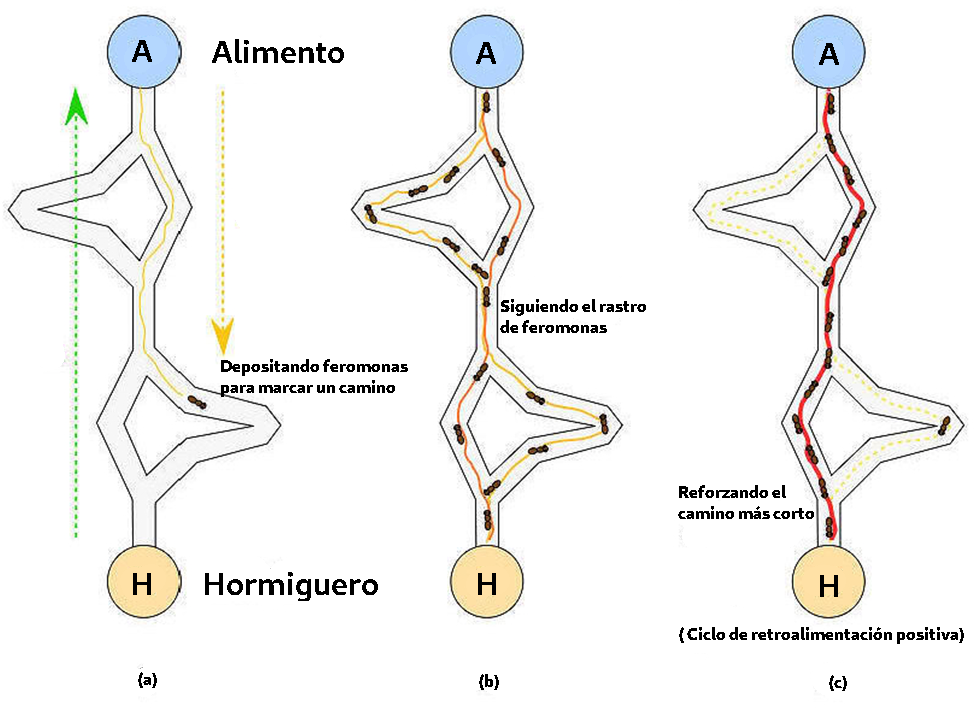
\includegraphics[scale=0.5]{imagenes/ACO-ant.png}
    \caption[Etapas de b\'usqueda de alimento y de comunicaci\'on entre hormigas.]{Etapas de b\'usqueda de alimento y de comunicaci\'on entre hormigas. (a) Flecha verde refleja la direcci\'on de la  b\'usqueda aleatoria, mientras que la flecha amarilla indica como una hormiga va depositando feromonas. (b) Otras hormigas siguen rastros de feromonas existente, aportando con sus propias feromonas. (c) Convergencia de las hormigas sobre el camino m\'as corto en base a la cantidad de feromonas depositada por m\'ultiples hormigas mediante un ciclo de retroalimentaci\'on positiva. Fuente: \citet{liu2020improving}.}
    \label{fig:hormigas}
\end{figure}
%Imagen de un recorrido

El conjunto de caminos que recorren las hormigas, para ir del hormiguero hacia la fuente de alimento y de retorno, puede ser interpretado como un grafo que representa esta red de caminos. En esta representaci\'on, la b\'usqueda de caminos corresponde a encontrar conjuntos de nodos o aristas adyacentes, y una componente de soluci\'on $c_{i}$ corresponde a una arista, siendo el recorrido desde una arista inicial hasta una arista final. La construcci\'on de una soluci\'on utiliza hormigas artificiales, tambi\'en llamadas agentes, que se desplazan a trav\'es del grafo mediante aristas adyacentes. La elecci\'on de aristas en cada paso de la construcci\'on utiliza la informaci\'on de las feromonas de cada una de las aristas candidatas, formando la soluci\'on incrementalmente. La metaheur\'istica ACO, indicada en el Algoritmo \ref{ACO-Algo}, consiste en 4 etapas, donde las 3 \'ultimas no tienen un orden espec\'ifico.

\begin{algorithm}[H]
\SetAlgoLined
 Ajuste de Par\'ametros \& inicializaci\'on de feromonas\;
 \While{Criterio de finalización no se cumple}{
   Construcci\'on\_de\_soluci\'on\_de\_cada\_hormiga()\;
   M\'etodo\_de\_b\'usqueda\_no\_local(); //Paso opcional\\
   Actualizaci\'on\_de\_feromonas()\;
 }
 \caption{Algoritmo metaheur\'istica ACO}\label{ACO-Algo}
\end{algorithm}


%%% CAMI VA AQUI

\subsection{Soluci\'on de un modelo COP mediante la metaheur\'istica ACO}

Un problema de optimización con restricciones, (COP, Constrained Optimization Problem) puede ser representado como $P = (S, \Omega, F)$, donde $S$ es el espacio de soluciones, $\Omega$ son las restricciones, y $F$ es la funci\'on objetivo. S esta definido por un conjunto discreto de variables $X = 1 \dotsc n$, con valores $v_{i}^{j} \in D_{i} = \{v_{i}^{1} \dotsc  v_{i}^{|D_{i}|}\}$. Se define como una variable {\it instanciada} la asignaci\'on a $X_i$ de un valor $v_{i}^{j} \in D_i$. Una solución candidata $s \in S$ es una soluci\'on factible si satisface las restricciones del conjunto $\Omega$. La funci\'on objetivo $F: S\rightarrow \mathbb R_{0}^{+}$, es la funci\'on de evaluaci\'on que asigna una puntuaci\'on a las soluciones candidatas. Al mismo tiempo, se define $s^{*}$ como una soluci\'on \'optima y $S^{*}$ como el conjunto que engloba todas las soluciones \'optimas, dado que pueden existir m\'ultiples soluciones $s^{*}$, y se relacionan mediante $s^{*} \in S^{*} \subseteq S $ \citepxl[ver\hspace{0.1cm} ]{socha2008ant}.
%Esta definici\'on permite aplicar la metaheur\'istica de optimizaci\'on basada en colonia de hormigas (ACO por su sigla en ingl\'es) a un modelo de un {\it COP}.
%COP es un CSP con función objetivo: https://en.wikipedia.org/wiki/Constrained_optimization#Constraint_optimization_problems

Es posible adaptar la definici\'on del modelo COP al modelo de feromonas de la metaheur\'istica ACO, mediante la asociaci\'on entre la definici\'on de variable {\it instanciada} del modelo COP y lo que representa un componente de soluci\'on o arista en un recorrido de una hormiga. 
Espec\'ificamente, si se extiende la definici\'on de componente de soluci\'on $c_{i}$ para que esta pueda tener valores $v_{i}^{j}$ que var\'ien dependiendo de un dominio $D_i$, el componente de soluci\'on pasa a ser $c_{ij}$. As\'i se obtiene la equivalencia entre la asignaci\'on $X_i = v_{i}^{j}$ que representa una variable {\it instanciada} del modelo COP, y la selecci\'on de un componente de soluci\'on $c_{ij}$,  para una soluci\'on o camino $s$ en ACO \citepxl{socha2008ant}.
%equivalente a una arista en esta investigaci\'on,


Luego, la definici\'on de una soluci\'on $s$ puede representarse como un conjunto de componentes de soluci\'on $c_{ij} \in C, i = 1 \dotsc n, j = 1 \dotsc |D_i|$. A su vez, la feromona asociada a una componente de soluci\'on se transforma de $\tau_i$ a $\tau_{ij}$. El Algoritmo  \ref{ACO-Algo} se modifica para representar la equivalencia entre el modelo COP y la metaheur\'istica ACO, a\~nadiendose las definiciones de los datos y el resultado esperado, quedando como lo indica el algoritmo \ref{COP-ACO-Algo}. 


\begin{algorithm}[H]
\SetAlgoLined
\KwData{Variables $X_i \dotsc X_n$, dominios $D_1 \dotsc D_n$, Restricciones $\in \Omega$}
\KwResult{conjunto s\textquotesingle $ \subseteq S$ != $\emptyset$, si existen soluciones factibles}
 Ajuste de Par\'ametros \& inicializaci\'on de feromonas \;
 \While{Criterio de finalización no se cumple}{
   Construcci\'on\_de\_soluci\'on\_de\_cada\_hormiga()\;
   M\'etodo\_de\_b\'usqueda\_no\_local(); //Paso opcional\\
   Actualizaci\'on\_de\_feromonas()\;
 }
 \caption{Algoritmo de un modelo COP adaptado a una metaheur\'istica ACO}\label{COP-ACO-Algo}
\end{algorithm}


% \section{Evaluaci\'on de t\'ecnicas}
% \label{sec:EvalOE4}

% Con el objetivo de profundizar la recopilaci\'on de informaci\'on sobre los m\'etodos presentados en las secciones \ref{sec:NonIndividualizationMethods} y \ref{sec:OptiMethods}, se realiza una evaluaci\'on de un representante de cada grupo. Debido a la complejidad al obtener informaci\'on cuantitativa de filamentos a partir de imagenes de microsco\'ia, las herramientas evaluadas a continuaci\'on pueden ofrecer soluciones que requieren una alta interacci\'on humana, o por otra parte conllevan un cierto grado de automatizaci\'on con el costo asociado de tener muchos par\'ametros. Ambas herramientas evaluadas presentan una versi\'on que los sucede, incorporando mejoras incrementales.

% mejoras incrementales de cada software

% \subsection{FibrilTool}
% \label{subsec:AnalisisFibrilTool}

% \subsection{SOAX}
% \label{subsec:AnalisisSOAX}